On previous sections every fragment of the system was described. Figure \ref{fig:System_Architecture} give a look to the common architecture of the system. The basic structure is composed of:

\begin{itemize}
  \item Set of quadrotors.
  \item Groundstation.
  \item Access Point (AP).
  \item Targets.
\end{itemize}

Every quadrotors has a camera and an embedded computer that runs the algorithm. Every frame, the algorithm segment the image and send to the ground station through the AP. The station process the received data and make an step on the tracking algorithm (EKF).

% System architecture image
\begin{figure}[hb]
	\centering
	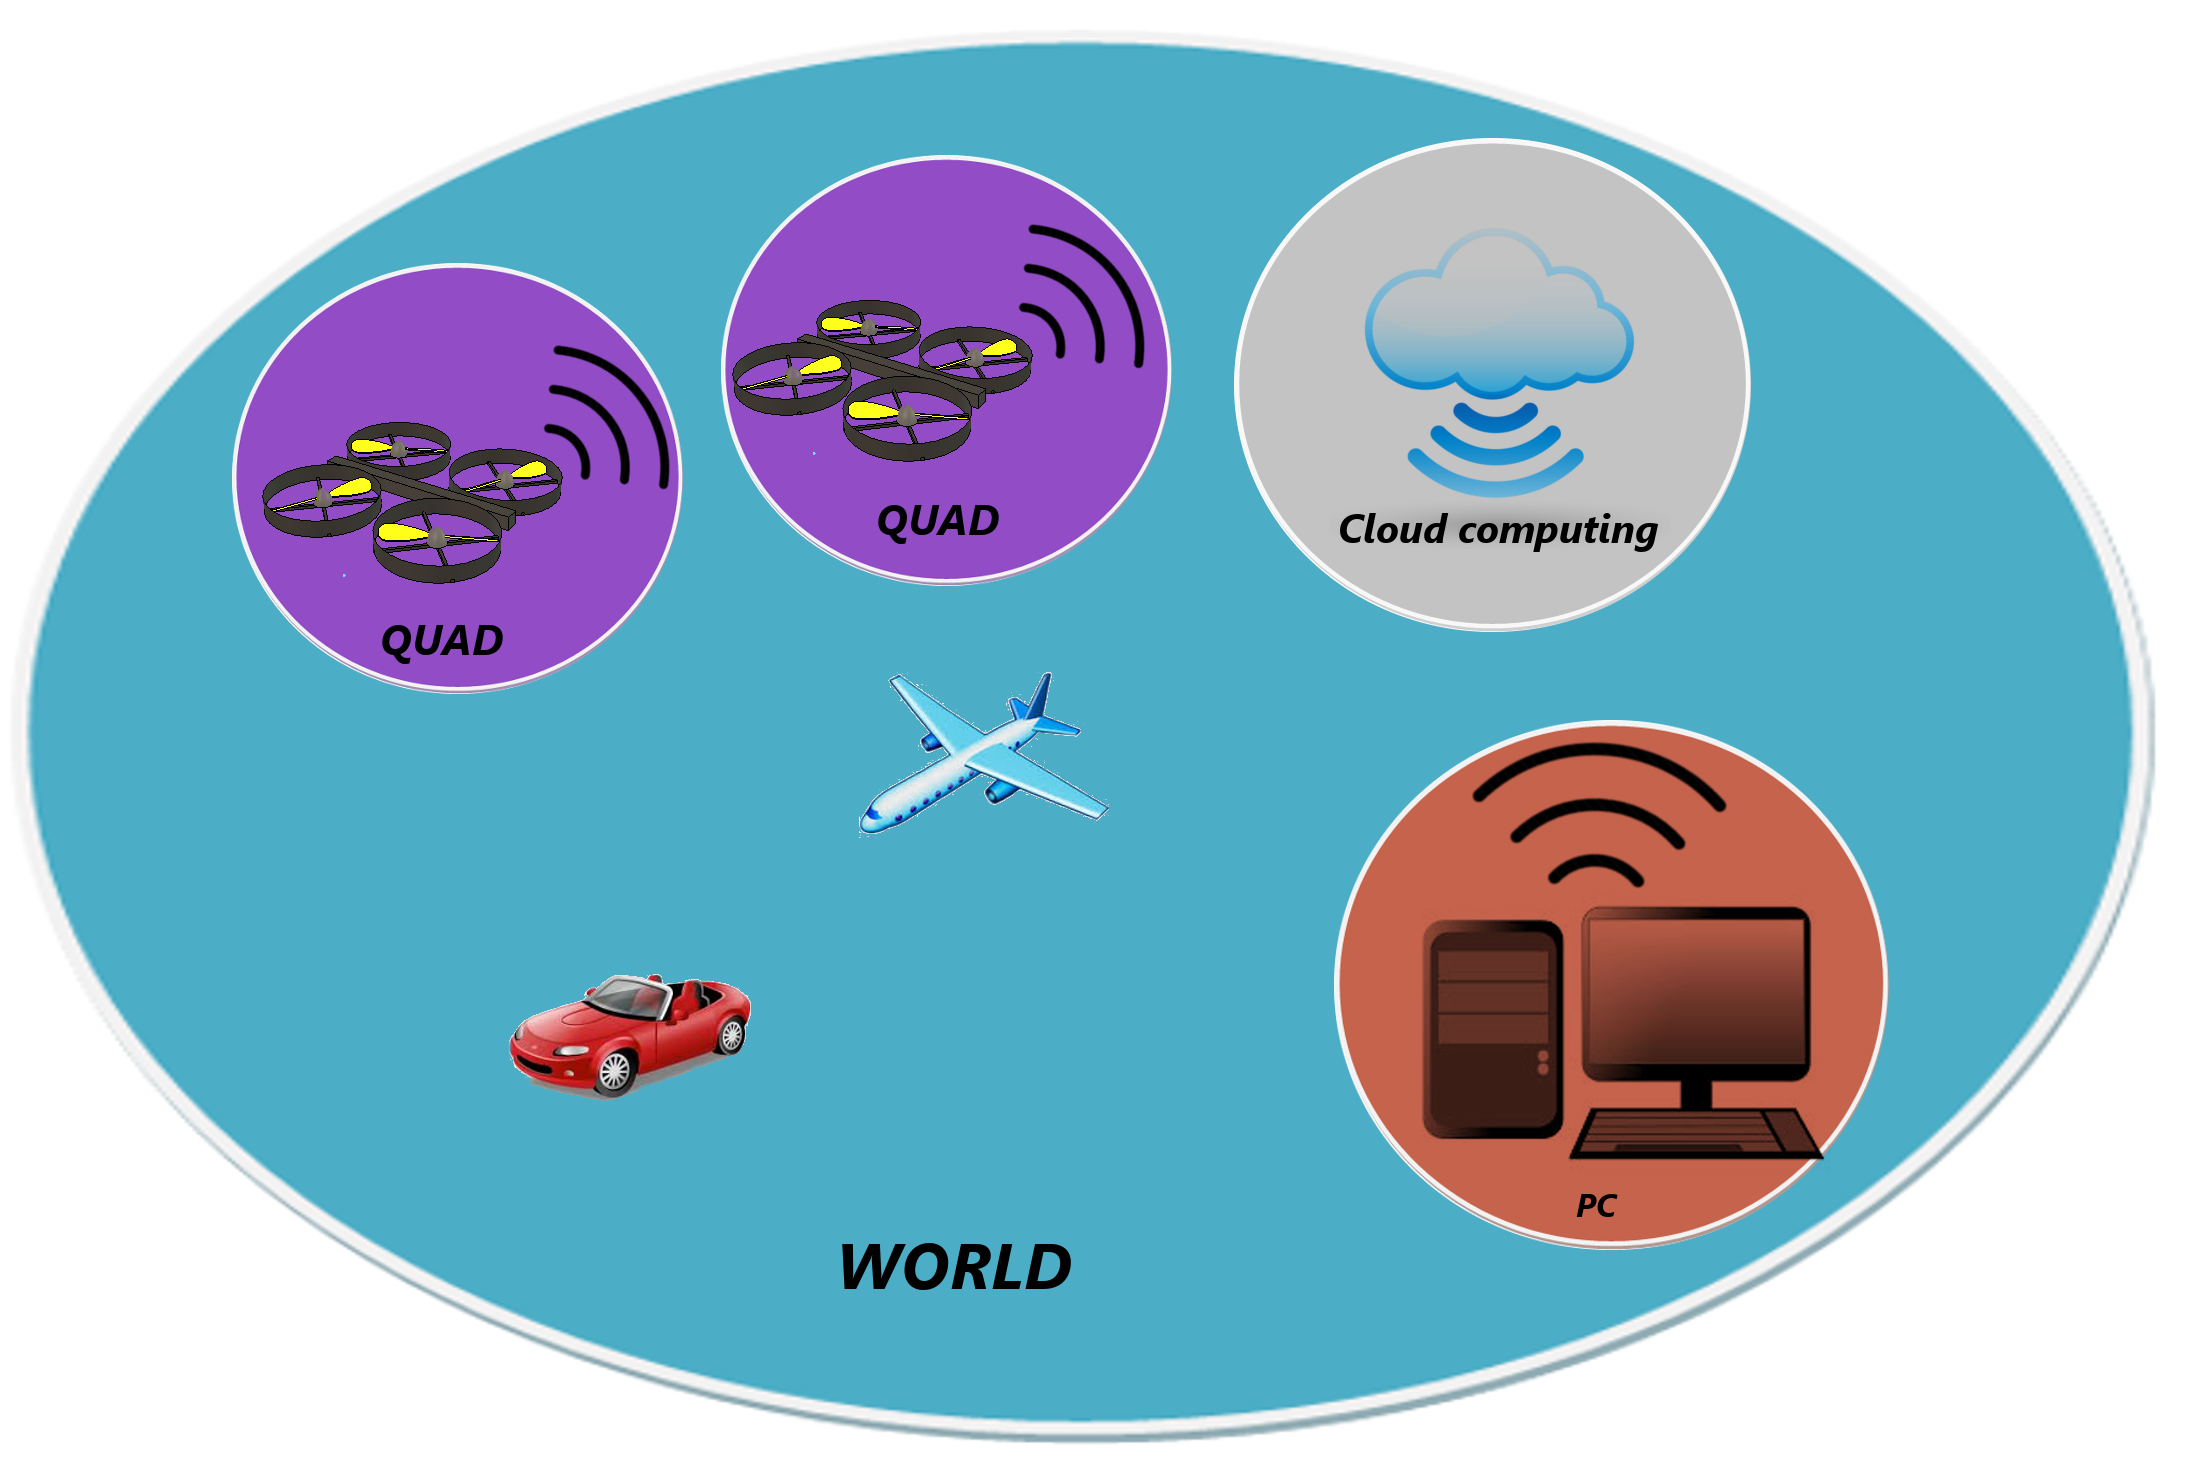
\includegraphics[width=0.50\textwidth,natwidth=220,natheight=1467]{../Images/c2/Architecture.png}
	\caption{System Architecture}
	\label{fig:System_Architecture}
\end{figure}

\subsection{Quadrotors Software}
	Every Quadrotor will run an application that is composed by a number of threads that allows it to parallelize the algorithm. This threads are:
	
	\begin{itemize}
		\item User interface thread.
		\item Image acquisition thread.
		\item Image segmentation thread.
		\item Communication thread.
	\end{itemize}
	% 666 TODO: terminar
	
\subsection{Ground Station Software}
	On the ground station, as in quad's computer, there will be running an application with parallel threads that manage the information to run as fast as possible the tracking algorithm. This threads are:
	
	
	\begin{itemize}
		\item User interface thread.
		\item Communication thread.
		\item Tracking thread.
	\end{itemize}
	% 666 TODO: terminar
	
\subsection{Conclusion}
The functionality of both quads and station can be easily modified by adding threads with access to the socket. For example, making the station to send the results of the EKF is as easier as send a message through the socket using the interface provided by BOViL \cite{BOViL}. 

In addition, the algorithm is designed with abstract interfaces from beginning, so any part of the architecture could be replaced by others with the same interface, for example:

\begin{itemize}
  \item Set of quadrotors $\Longrightarrow$ Set of quadrotors and ground vehicles.
  \item Ground Station $\Longrightarrow$ Multiple Ground Stations, cloud computation \cite{Cloud_computing} or even "inside quads" Station.
  \item Access Point (AP) $\Longrightarrow$ GSM modules (For cloud computing or if operation is far away from the Station).
  \item Targets.
\end{itemize}


% 666 TODO: terminar